\chapter{Integradores exponenciales y método de Linealización Local}\label{chapter:exp-int-and-ll-methods}

En este capítulo se presenta una revisión de la clase general de  integradores numéricos de tipo exponencial y de los Métodos de Linealización Local en particular, así como resultados básicos sobre el cálculo de la exponencial matricial.

En general, se considerarán los problemas de valor inicial definidos por los sistemas de $d$ ecuaciones diferenciales no autónomas de la forma
 \begin{equation}
 \frac{dx}{dt}=f(t,x), \;\; \label{ODE-SYST}
 \end{equation}
con condición inicial
 \begin{equation*}
 x(t_0)=x_0,
 \end{equation*}
 donde $x_0\in \mathfrak{D}$ es un vector columna de un conjunto abierto $\mathfrak{D}\subset\mathbb{R}^{d}$, $f: [t_0,T] \times \mathfrak{D}\longrightarrow \mathbb{R}^{d}$ es una función vectorial diferenciable y $t_0<T \in \mathbb{R}$. Se asumen condiciones de suavidad y condición de Lipschitz en $f$ para asegurar la unicidad de la solución en $\mathfrak{D}$. Denotaremos por $f_x$ la matriz Jacobiana de $f$ respecto a $x$ y por $f_t$ la derivada parcial de $f$ con respecto a $t$.

Consideremos, ademas, una partición $(t)_{h}={t_{n}:n=0,1,\ldots,N}$ del
intervalo $[t_{0},T]$ tal que $t_{0}<t_{1}<\ldots<t_{N}=T$, y $%
h_{n}=t_{n+1}-t_{n}\leq h$; para $n=0,\ldots,N-1$.

\section{Integradores exponenciales} \label{Sec:IE}

En general, se denomina integradores exponenciales a la familia
de esquemas numéricos para EDO que requieren del cálculo de algún término exponencial. Inicialmente, los integradores de este tipo comenzaron a desarrollarse en los años 60 del siglo pasado~\cite{Berland07} con el propósito de resolver sistemas de ecuaciones semilineales de la forma
\begin{equation}
\frac{dx(t)}{dt} = Ax(t) + F(x(t))  \;\;  \label{ODE Lines Method}
\end{equation}
que resultan de la discretización de una ecuación diferencial en derivadas parciales al utilizar el método de líneas, donde $A$ es una
matriz cuadrada, $F$ una función vectorial no lineal de $x(t)\in\mathbb{R}^d$ y $t\geq t_0 \in \mathbb{R}$. Típicamante, la matriz $A$ en (\ref{ODE Lines Method}) resulta mal condicionada, lo que establece un determinado nivel de rigidez (stiffness en inglés) para ese sistema de ecuaciones \cite{schiesser2012}. La rigidez del sistema (\ref{ODE Lines Method}) se incrementa con la disminución de la distancia entre los puntos de la discretización del método de líneas o con el aumento del número ecuaciones, lo que dificulta su integración con esquemas numéricos explícitos tradicionales \cite{schiesser2012}. Más recientemente, a finales de los años 90, la clase de integradores exponenciales fue extendida a EDO rígidas (stiff en ingles) de la forma general (\ref{ODE-SYST}).

Los integradores exponenciales tanto para ecuaciones semilineales (\ref{ODE Lines Method}) como para ecuaciones generales (\ref{ODE-SYST}) se derivan de aproximar la integral
que resulta de aplicar la fórmula de variación de constantes a estas ecuaciones~\cite{jimenez2020}. Al aplicar dicha fórmula la solución de la ecuación (\ref{ODE Lines Method}) se escribe como
\begin{equation}
x(t_n+h)=\me{Ah}\left(x(t_n) +\int\limits_{0}^{h} \me{-As}F(x(t_n+s)) \,ds\right)\,. \label{VCF2}
\end{equation}
Los integradores exponenciales obtenidos de aproximar esta expresión son, por ejemplo, los conocidos métodos de Lawson, Lawson Generalizados, Exponential Time
Differencing y Exponential Runge-Kutta (ver \cite{Berland07} para una revisión). Por otra parte, reescribiendo el campo vectorial de (\ref{ODE-SYST}) en la vecindad de ($t_n,x(t_n)$) como la suma de un término lineal y otro no lineal, la fórmula de variación de constantes lleva a
\begin{equation}
x(t_{n}+h) =  x(t_{n})+ \phi(t_{n},x(t_{n});h) + \bluemark{r(t_n,x(t_n);h)} \label{VCF-full}
\end{equation}
con
\begin{equation*}
 \phi(t_{n},x(t_{n});h) = \int\limits_{0}^{h}e^{A_{n}(h-s)}(f(t_n,x(t_{n}))+sf_t(t_n,x(t_{n})))ds 
\end{equation*}
y
\begin{equation}
 \bluemark{r(t_n,x(t_n);h)} =  \int\limits_{0}^{h}e^{A_{n}(h-s)}g_{n}(t_{n}+s,x(t_{n}+s))ds, \label{VCF}
\end{equation}
donde $A_{n}=f_x(t_n,x(t_{n}))$ es la matriz Jacobiana de $f$ evaluada en $(t_n,x(t_{n}))$,  $g_{n}(s,u)=f(s,u)-A_{n}(u-x(t_n))-f_t(t_n,x(t_{n}))(s-t_n)-f(t_n,x(t_n))$ es el término no lineal en la reescritura del campo vectorial de (\ref{ODE-SYST}) y $f_t$ es la derivada parcial de $f$ respecto a $t$. 
Ejemplos de integradores exponenciales obtenidos de aproximar esta expresión son el método clásico de Pope~\cite{pope1963exponential} de orden 2, los métodos Runge-Kutta Localmente 
Linealizados~\cite{delaCruz06,Jimenez13,Jimenez14AMC}, los métodos Exponenciales de Propagación 
Iterativa~\cite{tokman2006efficient, tokman2012new}, los métodos de Taylor Localmente Linealizados~\cite{delaCruz07}, los
métodos Exponenciales tipo Rosenbrok~\cite{hochbruck2009exponential} y los métodos Exponenciales tipo Adams~\cite{hochbruck2011exponential}, todos de orden superior a 2.

En el contexto de las ecuaciones diferenciales de dimensiones pequeñas los integradores exponenciales también fueron tempranamente introducidos como aproximación a las soluciones de dichas ecuaciones. Por ejemplo, para aproximar las ecuaciones diferenciales estocásticas~\cite{ozaki19852,ozaki1985statistical} y sus asociados problemas de filtrado continuo-discreto~\cite{ozaki1993local} y estimación de procesos de difusión~\cite{ozaki19852,ozaki1985statistical,ozaki1994local}. Luego fueron extendidos para la integración de ecuaciones diferenciales aleatorias~\cite{carbonell2005local}, con retardo~\cite{jimenez2006local} y para las parciales estocásticas semilineales~\cite{jentzen2009overcoming,kloeden2011exponential}.

En general, los integradores exponenciales tienen en cuenta que una parte significativa de la estabilidad y las propiedades dinámicas de las ecuaciones diferenciales está contenida en la linealización de la ecuación tratada y se constituyen como una alternativa importante a los métodos implícitos para resolver ecuaciones diferenciales rígidas~(\textit{stiff} en inglés) o altamente oscilatorias.  


\section{Método de Linealización Local}\label{section:ll-methods}
En esta sección se presentan los resultados básicos los Métodos de Linealización Local que se requieren para esta tesis.

\subsection{Aproximación Lineal Local}

El método clásico de Linealización Local de orden 2 de Pope~\cite{pope1963exponential}
 consiste en aproximar en cada paso el campo vectorial de (%
\ref{ODE-SYST}) mediante la expansión de Taylor de primer orden, para
luego resolver exactamente la ecuación lineal resultante. Más
precisamente, si $A_{n}y(t)+a_{n}(t)$ denota la aproximación de Taylor
de primer orden de $f$ en una vecindad de $(t_n,y_{n})$, donde \mbox{$
	A_{n}=f_{x}(t_n,y_{n})$} y $a_{n}(t)=f(t_n,y_{n})-A_{n}y_{n}+f_t(t_n,y_n)(t-t_n)$, entonces la
solución de la ecuación 
\begin{eqnarray}
\frac{dy}{dt} & = & A_{n}y+a_{n}(t) \label{ODE-SYST-LINEAL-1} \\
y(t_{n})& = & y_{n}  \nonumber
\end{eqnarray}
para todo $t\in[t_{n},t_{n+1}]$ es una aproximación de la solución
de (\ref{ODE-SYST}) con condición inicial \mbox{$x(t_{n})=y_{n}$}. Mediante la fórmula de variación de constantes obtenemos 
\begin{equation*}
y(t)=y_{n}+\phi(t_{n},y_{n};t-t_{n}),  %\label{ODE-SYST-FORM-LL}
\end{equation*}
donde 
\begin{equation}
\phi(t_{n},y_{n};t-t_{n})=\int\limits^{t-t_{n}}_{0} e^{{A_{n}(t-t_{n}-u)}}
(A_{n}y_{n}+a_{n}(t_{n}+u))\,du.  \label{REV-PHI-DEF-2}
\end{equation}
Aplicando recursivamente la expresión anterior obtenemos la siguiente
definición.

\importantdefinition{Discretización Lineal Local}
\begin{definition}
	\label{definition LLD} Dada una partición $(t)_{h}$, la discretización Lineal Local de la solución de (\ref{ODE-SYST}) está dada por la expresión recursiva
	\begin{equation}
	y_{n+1}=y_{n}+\phi \left( t_{n},y_{n};h_{n}\right) ,  \label{ODE-LLA-4}
	\end{equation}%
	con $y_{0}=x_{0}$, $n=0,1,\ldots,N-1$ y $\phi$ definida en (\ref{REV-PHI-DEF-2}).
\end{definition}

Para todo $t\in[t_{0},T]$ se define la siguiente aproximación.
\importantdefinition{Aproximación Lineal Local}
\begin{definition}
	\label{definition LLA} Dada una partición $(t)_{h}$, la aproximación
	Lineal Local de la solución de (\ref{ODE-SYST}) está dada por 
	\begin{equation}
	y(t)=y_{n_{t}}+\phi(t_{n_{t}},y_{n_{t}};t-t_{n_{t}})
	\label{ODE-REV-FORM-LLA}
	\end{equation}
	para todo $t\in[t_{0},T]$, donde $y_{0}=x_{0}$, $y_{n_{t}}$ es la discretización Lineal Local (\ref{ODE-LLA-4}) y ${n_{t}=\maxx{n:t_{n}\leq t}}$.
\end{definition}
%Otros  integradores que provienen de esta aproximación son~\cite{Jimenez02AMC,Jimenez05AMC}.

 La convergencia, la estabilidad lineal y varias propiedades dinámicas de  la discretización Lineal Local (\ref{ODE-LLA-4}) se pueden encontrar en \cite{Jimenez02AMC}. 
 
 Obsérvese que $\phi$ en la discretización Lineal Local (\ref{ODE-LLA-4}) representa la primera integral de la expresión (\ref{VCF-full}) y que, con $y_n=x(t_n)$, la discretización Lineal Local (\ref{ODE-LLA-4}) coincide con los dos primeros términos de la expresión (\ref{VCF-full}). De esta forma la integral de la expresión (\ref{VCF}) representa el residuo de la aproximación (\ref{ODE-LLA-4}) a la solución de la ecuación diferencial (\ref{ODE-SYST}) en $t_{n+1}=t_n+h$.
\subsection{Aproximación Lineal Local de Orden Superior}

La estabilidad y las propiedades dinámicas que la discretización Lineal Local (\ref{ODE-LLA-4}) posee son de vital importancia para la integración de EDO, no obstante su bajo orden de convergencia constituye una limitante en algunas circunstancias. Para solucionar esa dificultad se construyen los métodos de Linealización Local de Orden Superior~(LLOS) los cuales retienen las propiedades mencionadas, pero con orden de convergencia mayor. 

Estos métodos de Linealización Local de Orden Superior se obtienen de agregar a la aproximación Lineal Local~(\ref{ODE-REV-FORM-LLA}) un término adicional $\widetilde{r}$ que resulta de aproximar, con un orden superior a 2, la integral de la expresión~(\ref{VCF}) por algún método de cuadratura o por la solución numérica de la representación diferencial de la integral~(\ref{VCF})~\cite{delaCruz06}. \bluemark{Utilizando} diferentes tipos de cuadraturas para aproximar~(\ref{VCF}) se obtienen los métodos Exponenciales de Propagación 
Iterativa~\cite{tokman2006efficient}, los métodos de Taylor Localmente Linealizados~\cite{delaCruz07}, los
métodos Exponenciales tipo Rosenbrok~\cite{hochbruck2009exponential} y los métodos Exponenciales tipo Adams~\cite{hochbruck2011exponential}. Por otra parte, \bluemark{utilizando} esquemas Runge Kutta (RK) para resolver la mencionada ecuación diferencial se obtienen los métodos Runge-Kutta Localmente Linealizados~\cite{delaCruz06,Jimenez13,Jimenez14AMC}.

Por su relevancia en esta tesis, a continuación se expondrá con mas detalle los métodos Runge-Kutta Localmente Linealizados. 
\importantdefinition{Aproximación Lineal Local de Orden Superior}
Dada una partición $(t)_{h}$, una aproximación Lineal Local de orden $%
\gamma$ de la solución de (\ref{ODE-SYST}) se define por la expresión~\cite{Jimenez13}
\begin{equation}
y(t)=y_{n_{t}}+\phi(t_{n_{t}},y_{n_{t}};t-t_{n_{t}})+\widetilde{r}(t,t_{n_{t}},y_{n_{t}}),
\label{ODE-REV-HOLL}
\end{equation}
donde ${n_{t}=\maxx{n:t_{n}\leq t}}$, $\widetilde{r}(t,t_{n_{t}},y_{n_{t}})$ es la solución numérica de orden $\gamma >2$ de la \bluemark{representación diferencial de la integral~(\ref{VCF})}
\begin{eqnarray}
\frac{dr}{dt} & = & q(t_{n},y_{n},t,r(t))  \label{ODE r} \\
r(t_{n}) & = & 0 \nonumber
\end{eqnarray}
para todo $t\in [t_{n},t_{n+1})$, con campo vectorial 
\begin{eqnarray*}
q(t_n,y_n,s,\varsigma)&=&f(s,y_n+\phi(t_n,y_n;s-t_n)+\varsigma)-f_x(t_n,y_n)\phi(t_n,y_n;s-t_n)\\
 & &-f_t(t_n,y_n)(s-t_n) -f(t_n,y_n) ,
%\label{AUX-ODE}
\end{eqnarray*}
para todo $s\in [t_{n},t_{n+1})$ y $\varsigma \in \mathbb{R}^d $. Aquí, la ecuación (\ref{ODE r}) resulta de derivar (\ref{VCF}) con respecto a t. 

Cuando $\widetilde{r}$ en (\ref{ODE-REV-HOLL})  es la aproximación obtenida mediante un esquema Runge-Kutta de orden $\gamma$ se llega a las definiciones siguientes.
\importantdefinition{Discretización Lineal Local Runge-Kutta}
\begin{definition}
	\label{definition HLLD} \cite{Jimenez13} Dada una partición $(t)_{h}$, la discretización Lineal Local Runge-Kutta 
    de orden $\gamma >2$ se define por la expresión recursiva:
	\begin{equation*}
	y_{n+1}=y_{n}+\phi \left( t_{n},y_{n};h_{n}\right) +h_{n}\sum_{j=1}^{s}b_{j}\kt_{j}(t_n,y_n,h_n)
	%\label{LLRK_Discretizat}
	\end{equation*}%
	con $y_{0}=x_{0}$, donde las constantes $b_{j}$ y las funciones $k_{j}$ están definidas por el método Runge-Kutta de $s$ estados aplicado a la ecuación~(\ref{ODE r}).
\end{definition}
\importantdefinition{Aproximación Lineal Local Runge-Kutta}
\begin{definition}
	\label{definition HOLLA} \cite{Jimenez13} Dada una partición $(t)_{h}$, la aproximación Lineal Local Runge-Kutta de orden $\gamma$ se define por 
	\begin{equation*}
	y(t)=y_{n_{t}}+\phi(t_{n_{t}},y_{n_{t}};t-t_{n_{t}})+(t-t_{n_{t}})%
	\sum_{j=1}^{s}b_{j}\kt_{j}(t_{n_{t}},y_{n_{t}},t-t_{n_{t}}) %\label{LLRK_Approx}
	\end{equation*}
	para todo $t\in[t_{0},T]$, donde $y_{n_{t}}$ es la discretización Lineal Local Runge-Kutta de orden $\gamma$, y $n_{t}=\maxx{n:t_{n}\leq t}$.
\end{definition}

Como ejemplos importantes se tienen las siguientes discretizaciones Lineales Locales Runge-Kutta de orden 4 y 4-5.

Utilizando la fórmula Runge-Kutta clásica de orden 4~\cite{hairer1993solving} para integrar la ecuación auxiliar (\ref{ODE r}), se obtiene la discretización Lineal Local Runge-Kutta de orden 4~\cite{Jimenez13}:

\begin{equation}
    y_{n+1}\,=\,y_n+\phi(t_n,y_n;h_n)+\frac{h_n}{6}(2\kt_2+2\kt_3+\kt_4)
    \label{LL-scheme-4}
\end{equation}
con
    \[ \kt_j = f\left( t_n+c_jh_n\, , \, y_n+\phi(t_n,y_n;c_jh_n)+c_jh_n\kt_{j-1} \right)
- f_x(t_n\, , \, y_n)\phi(t_n,y_n;c_jh_n) - f(t_n\, ,\, y_n) ,\]
donde $\kt_1=0$ y $c = \left[ 0 \; \frac{1}{2} \; \frac{1}{2} \; 1  \right]$.

Si se utilizan las fórmulas embebidas Runge-Kutta de Dormand y Prince para integrar la ecuación auxiliar (\ref{ODE r}), entonces se obtiene la discretización embebida Lineal Local Runge-Kutta~\cite{Jimenez14AMC}
\begin{equation}
y_{n+1}\,=\,y_n+\phi_s+h_n \sum_{j=1}^{s}b_j \kt_j \quad \text{y} \quad
\widehat{y}_{n+1}\,=\, y_n+\phi_s+h_n \sum_{j=1}^{s}\widehat{b}_j \kt_j
\label{LLDP-scheme-dp}
\end{equation}
de orden 5 y 4, donde $s = 7$ es el número de estados,
\[ \kt_j = f\left( t_n+c_jh_n\, , \, y_n+\phi_j+h_n \sum_{i=1}^{j-1}a_{j,i}\kt_i \right)  
- f_x(t_n\, , \, y_n)\phi_j - f(t_n\, ,\, y_n),\]
\[ \phi _j = \phi \left( t_{n},y_{n};c_jh_{n}\right), \]
y coeficientes Runge-Kutta $a_{j,i}$, $b_j$, $\hat{b}_j$ y $c_j$ definidos en Tabla \ref{ButcherTabla}.


\begin{table}[h]
	\caption{Butcher tableau para los coeficientes de las fórmulas Runge-Kutta embebidas de Dormand y Prince~\cite{hairer1993solving}} \label{ButcherTabla}
	\begin{center}
		\begin{tabular}{ l@{\vrule height 5pt depth 10pt width 0pt}|lllllll}
			$0$ & \\
			$\frac{1}{5}\quad$ & $\frac{1}{5}$ \\
			$\frac{3}{10}\quad$ & $\frac{3}{40}$ & $\frac{9}{40}$ \\
			$\frac{4}{5}\quad$ & $\frac{44}{45}$ & $-\frac{56}{15}$ & $\frac{32}{9}$ \\
			$\frac{8}{9}\quad$ & $\frac{19372}{6561}$ & $-\frac{25360}{2187}$ & $\frac{64448}{6561}$ & $-\frac{212}{729}$ \\
			$1\quad$ & $\frac{9017}{3168}$ & $-\frac{355}{33}$ & $\frac{46732}{5247}$ & $\frac{49}{176}$
			& $-\frac{5103}{18656}$ \\
			$1\quad$ & $\frac{35}{384}$ & $0$ & $\frac{500}{1113}$ & $\frac{125}{192}$
			& $-\frac{2187}{6784}$ & $\frac{11}{84}$ \\
			\hline
			$\widehat{y}$ & $\frac{5179}{57600}$ & $0$ & $\frac{7571}{16695}$ & $\frac{393}{640}$
			& $-\frac{92097}{339200}$ & $\frac{187}{2100}$ & $\frac{1}{40}$
			\rule[-0.3cm]{0cm}{0.8cm} \\
			$y$ & $\frac{35}{384}$ & $0$ & $\frac{500}{1113}$ & $\frac{125}{192}$
			& $-\frac{2187}{6784}$ & $\frac{11}{84}$ & $0$
		\end{tabular}
	\end{center}
\end{table}

En síntesis, a la clase de métodos de Linealización Local de Orden Superior pertenecen los integradores numéricos derivados de dividir, en intervalos de tiempo consecutivos, la solución $x$ de la ecuación original en dos partes: la solución $u$ de la ecuación linealizada localmente más una solución aproximada a la representación diferencial del residuo $r = x-u$ proporcionada por un integrador numérico de orden alto. La Figura \ref{fig:ll-graph} muestra una representación gráfica de esta explicación. 


%\begin{figure}[ht]
%	% \centering
%	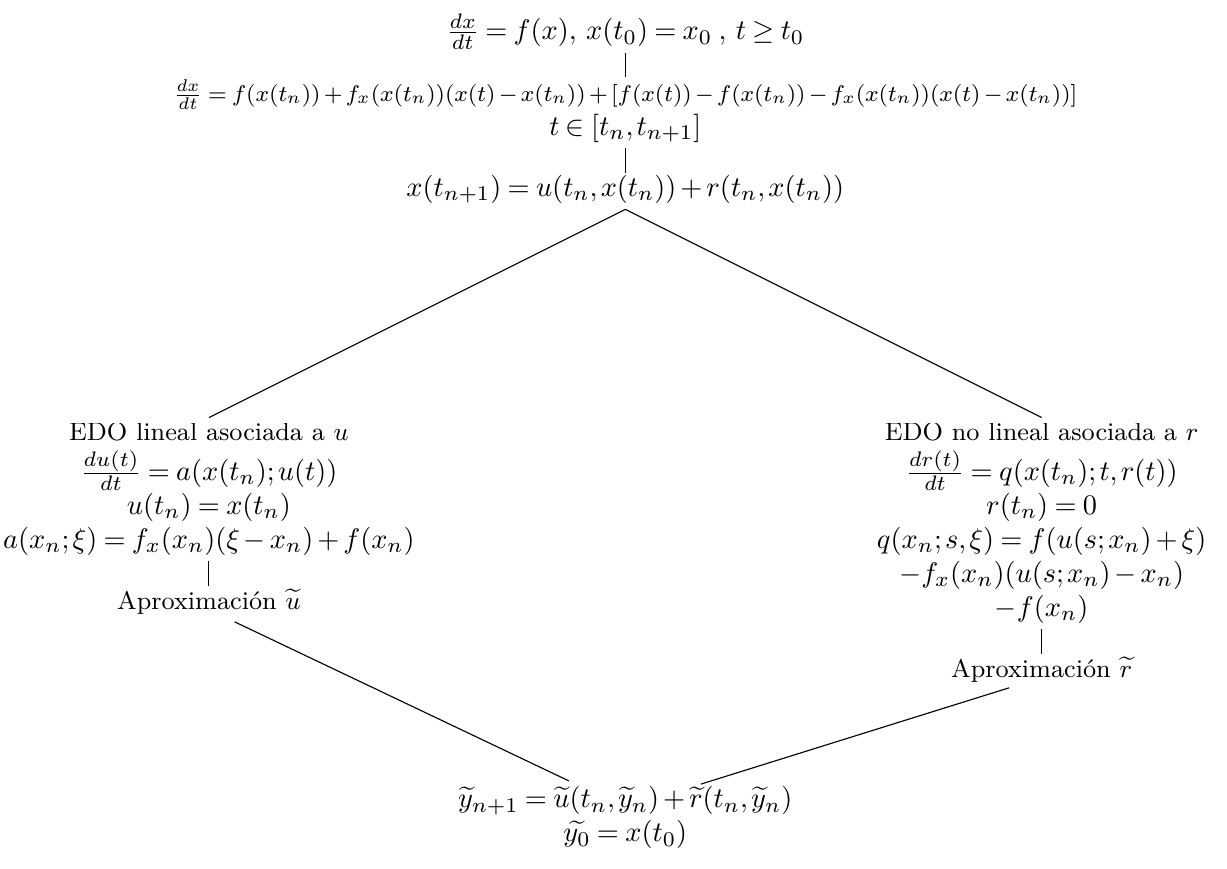
\includegraphics[scale=0.55]{Graphics/diagram-ll.jpg}
%	\caption{Representación gráfica de la descomposición Lineal Local (\ref{VCF-full}) de la solución x de una ecuación diferencial ordinaria, y de un esquema de  Linealización Local de Orden Superior $\widetilde{y}_{n+1}$.}
%	\label{fig:ll-graph}
%\end{figure}

\begin{figure}[htb]
%	\qtreeshowframes
	\begin{center}
		\leaf{\small \tikzmark{c} Aproximación $\widetilde{u}$  \tikzmark{d} }
		\branch{1}{\small EDO lineal asociada a $u$\\$\frac{du(t)}{dt} = a(x(t_n);u(t))$\\$u(t_n)=x(t_n)$\\$a(x_n;\xi) = f_x(x_n)(\xi-x_n)+f(x_n)$}
		\brOverride
		\leaf{ \tikzmark[top]{a} $\widetilde{y}_{n+1} = \widetilde{u}(t_{n},\widetilde{y}_n)+\widetilde{r}(t_{n},\widetilde{y}_n)$  \tikzmark[top]{b}\\
		$\widetilde{y_0}=x(t_0)$}
		\branch{1}{ \\ \\ \\ \\ \\ \\ \\ \\ \\ \\}
		\brRestore
		\leaf{\small \tikzmark{e} Aproximación $\widetilde{r}$ \tikzmark{f}}
		\branch{1}{\small EDO no lineal asociada a $r$\\$\frac{dr(t)}{dt} = q(x(t_n);t,r(t))$\\$r(t_n)=0$\\
			$q(x_n;s,\xi)=f(u(s;x_n)+\xi)$\\
			 $-f_x(x_n)(u(s;x_n)-x_n)$\\
			$-f(x_n)$
		}
		\brOverridedd
		\branch{3}{$ x(t_{n+1}) = u(t_{n},x(t_n))+r(t_{n},x(t_n))$}
		\brRestore
		\branch{1}{\footnotesize $\frac{dx}{dt}=f(x(t_n))+f_x(x(t_n))(x(t)-x(t_n))+\left[ f(x(t))-f(x(t_n))-f_x(x(t_n))(x(t)-x(t_n))  \right]$\\$ t\in[t_{n},t_{n+1}]$}
		\branch{1}{$\frac{dx}{dt}=f(x),\; x(t_0)=x_0\;,\; t\geq t_0$}
		\qobitree
	\end{center}
	\begin{tikzpicture}[overlay, remember picture]
		\draw [-, shorten >=22pt, shorten <=10pt] ($(pic cs:c)!1/2!(pic cs:d)$) -- ($(pic cs:a)!1/2!(pic cs:b)$);
		\draw [-, shorten >=28pt, shorten <=12pt] ($(pic cs:e)!1/2!(pic cs:f)$) -- ($(pic cs:a)!1/2!(pic cs:b)$);
	\end{tikzpicture}
	\caption{Representación gráfica de la descomposición Lineal Local (\ref{VCF-full}) de la solución x de una ecuación diferencial ordinaria, y de un esquema de  Linealización Local de Orden Superior $\widetilde{y}_{n+1}$.}
	\label{fig:ll-graph}
\end{figure}


\subsection{Esquemas de Linealización Local}

Como puede notarse de las Definiciones \ref{definition LLD} y \ref{definition HLLD} , las
discretizaciones Lineales Locales no pueden ser implementadas directamente por
estar expresadas en término de integrales o ecuaciones diferenciales que en general no pueden ser
calculadas analíticamente. Dependiendo de la forma de calcular  numéricamente esas integrales,
 diferentes esquemas numéricos pueden ser obtenidos \cite{Jimenez05AMC,Jimenez13}.
 Más precisamente tenemos la siguiente definición.
 \importantdefinition{Esquema de Linealización Local}
\begin{definition}
	\label{definition LLS} Dada la discretización Lineal Local 
	  $y_n=y_{n}+\digamma(t_{n},y_{n},t-t_{n})$
	 de orden $\gamma $, toda fórmula recursiva de la forma 
	\begin{equation*}
	 \widetilde{y}_{n+1}=\widetilde{y}_{n}+\widetilde{\digamma}(t_{n},\widetilde{y}_{n},t-t_{n})
	 , \text{ \ \ \ \
		\ con }\widetilde{y}_{0}=y_{0},
	\end{equation*}%
	donde $\widetilde{\digamma}$ denota una aproximación
	de $\digamma$ mediante un algoritmo numérico, es
	llamada genéricamente esquema de Linealización Local (LL).
\end{definition}
\importantdefinition{Esquema de Linealización Local de Orden Superior}
Regularmente, en la literatura, la implementación numérica de la discretización Lineal Local~(\ref{ODE-LLA-4}) se denomina simplemente esquema de Linealización Local, mientras que la implementación numérica de una aproximación de orden superior como la~(\ref{ODE-REV-HOLL}) se denomina esquema de Linealización Local de Orden Superior (LLOS).

Por ejemplo, cuando la fórmula de Padé con escalamiento y potenciación para exponenciales matriciales \cite{moler2003nineteen} es utilizada para
aproximar $\phi$ en la discretización Lineal Local~(\ref{ODE-LLA-4}) se obtiene el esquema LL de orden $2$ \cite{Jimenez02AMC}
\begin{equation} 
\widetilde{y}_{n+1}=\widetilde{y}_{n}+\widetilde{\phi}\left( t_{n},\widetilde{y}_{n};h_{n}\right), \label{LL-scheme}
\end{equation} 
donde $\widetilde{\phi }\left( t_{n},\widetilde{y}
_{n},h_{n}\right) =\lmatrix\,(P_{\pf,\qf}(2^{-k_{n}}\widetilde{M}_{n}h_{n}))^{2^{k_{n}}}\rvector$, 
$(P_{\pf,\qf}(2^{-k_{n}}\widetilde{M}_{n}h_{n}))^{2^{k_{n}}}$ es la aproximación
de Padé de orden $(\pf,\qf)$ de  $\me{\widetilde{M}_{n}h_{n}}$, $k_{n}$ es el menor número natural tal que $\left\Vert 2^{-k_{n}}\widetilde{M}_{n}h_{n}\right\Vert \leq \frac{1}{2}$ 
y las matrices $\widetilde{M}_{n}$, $\lmatrix$, $\rvector$ están definidas como

\begin{equation*}
\widetilde{M}_{n}=\left[ 
\begin{array}{ccc}
f_{x}(t_{n},\widetilde{y}_{n}) &f%
_{t}(t_{n},\widetilde{y}_{n}) & f(t_{n},\widetilde{
		y}_{n}) \\ 
0 & 0 & 1 \\ 
0 & 0 & 0%
\end{array}%
\right] \in \mathbb{R}^{(d+2)\times (d+2)},
\end{equation*}%
$\lmatrix=\left[ 
\begin{array}{ll}
I_{d} & 0_{d\times 2}%
\end{array}%
\right] $ y $\rvector^{\intercal }=\left[ 
\begin{array}{ll}
\mathbf{0}_{1\times (d+1)} & 1%
\end{array}%
\right] $ para EDO no autónomas; y 
\begin{equation*}
\widetilde{M}_{n}=\left[ 
\begin{array}{cc}
f_{x}(\widetilde{y}_{n}) & f(\widetilde{y}_{n}) \\ 
0 & 0%
\end{array}%
\right] \in \mathbb{R}^{(d+1)\times (d+1)},
\end{equation*}%
$\lmatrix=\left[ 
\begin{array}{ll}
I_{d} & 0_{d\times 1}%
\end{array}%
\right] $ y $\rvector^{\intercal }=\left[ 
\begin{array}{ll}
\mathbf{0}_{1\times d} & 1%
\end{array}%
\right] $ para ecuaciones autónomas.

Por otra parte, cuando la mencionada aproximación de Padé se utiliza para aproximar $\phi$ y $\phi_j$ en las discretizaciones~(\ref{LL-scheme-4}) y~(\ref{LLDP-scheme-dp}) se obtienen los esquemas LLOS propuestos en \cite{Jimenez13,Jimenez14AMC} orientados a resolver problemas de valor inicial de dimensiones pequeñas. La Figura \ref{fig:ll-graph} muestra una representación gráfica resumida de como se construyen esquemas LLOS en general. 

\section{Cálculo de la exponencial de una matriz}

\begin{definition}
    \label{EXPM}\cite{golub2013matrix} Sea $A$ una matriz de $n\times n$ real o compleja. La exponencial de $A$ denotada por
    $ \me{A} $ o $\mathrm{exp}(A)$ es una matriz de $n\times n$ dada por la serie de potencias
    \[\me{A}=\sum_{k=0}^{\infty}\frac{1}{k!}A^{k}.\]
\end{definition}
En muchas aplicaciones se utiliza $\me{tA}$ donde $t$ es un escalar, por tanto 
\begin{equation}
\me{tA}=I+tA+\frac{t^{2}A^{2}}{2!}+\cdots\label{EXPM-SERIE}
\end{equation}
\begin{theorem}\cite{IntroMatrix}
    La serie de matrices definida en~(\ref{EXPM-SERIE}) existe para toda matriz $A$ para $t$ fijo y
    para todo $t$ para $A$ fija. La serie converge uniformemente en cualquier región de t del plano complejo.
\end{theorem}

En \cite{moler2003nineteen} se presenta una revisión de los métodos numéricos
para aproximar
la exponencial de matrices. Los métodos más utilizados son la aproximación de Padé con escalamiento
y potenciación para matrices pequeñas y densas, y el de los subespacios de Krylov para matices grandes y esparcidas.


\subsection{Aproximación de Padé}\label{section:pade-approx}
\importantdefinition{Aproximación de Padé}
\begin{definition}
    \cite{golub2013matrix}~La aproximación racional de Padé $P_{\pf,\qf}(z)$
    de $\me{z}$ está dada por 
    \begin{equation*}
    P_{\pf,\qf}(z)=D_{\pf,\qf}(z)^{-1}N_{\pf,\qf}(z),  \label{FORM PADE}
    \end{equation*}%
    donde 
    \[
    N_{\pf,\qf}(z)=\sum\limits_{k=0}^{\pf}\frac{(\pf+\qf-k)!\pf!}{(\pf+\qf)!k!(\pf-k)!}z^k
    \]%
    y 
    \[
    D_{\pf,\qf}(z)=\sum\limits_{k=0}^\qf\frac{(\pf+\qf-k)!\qf!}{(\pf+\qf)!k!(\qf-k)!}(-z)^k
    \]
\end{definition}

Cuando la norma de \mmark{una} \redmark{matriz cuadrada} $A$ es grande, el costo computacional y los errores de redondeo \mmark{en $P_{\pf,\qf}(A)$} aumentan, por lo que
es necesaria la alternativa de escalamiento y potenciación.

\begin{definition}\cite{golub2013matrix}~
    Sea $A$ una matriz cuadrada, y sea $P_{\pf,\qf}(2^{-k}A%
    )$ la aproximación de Padé de orden $(\pf,\qf)\ $de $\me{2^{-k}A%
    }$, donde $k$ es el menor número natural tal que $\left\vert 2^{-k}A%
    \right\vert \leq \frac{1}{2}$. \ Se define la aproximación de  Padé-$(\pf,\qf)$ con escalamiento y potenciación como 
    \begin{equation}
    F_{k}^{\pf,\qf}(A)=(P_{\pf,\qf}(2^{-k}A))^{2^{k}}.
    \label{P-MA-2}
    \end{equation}
\end{definition}

Resultados sobre el error y la estabilidad de las aproximaciones de Padé se presentan a continuación.

\begin{theorem}
    \label{Conv. Pade}\cite{jimenez2012convergence} El error
    relativo y absoluto de la aproximación de Padé con escalamiento y
    potenciación (\ref{P-MA-2}) de $\me{A}$ está dado por: 
    \[
    \frac{\left\vert e^{A}-F_{k}^{\pf,\qf}(A)\right\vert 
    }{\left\vert e^{A}\right\vert }\leq \epsilon _{p,q}\left\vert 
    A\right\vert e^{\epsilon _{p,q}\left\vert A\right\vert }
    \]%
    y 
    \begin{equation}
    \left\vert \me{A}-F_{k}^{\pf,\qf}(A)\right\vert \leq
    c_{p,q}(k,\left\vert A\right\vert )\left\vert A\right\vert
    ^{p+q+1}, \label{errpade}
    \end{equation}
    donde $\epsilon _{p,q}=\alpha (\frac{1}{2})^{p+q-3}$, $%
    c_{p,q}(k,\left\vert A\right\vert )=\alpha
    2^{-k(p+q)+3}\me{(1+\epsilon _{p,q})\left\vert A\right\vert }$ y $%
    \alpha =\frac{p!q!}{(p+q)!(p+q+1)!}$.
\end{theorem}

\begin{theorem}\label{Stab. Pade}[Teorema 4.12 en \cite{wanner1996solving}] 
    La aproximación de Padé $P_{\pf,\qf}(z)$  es \emph{A-estable} si y solo si $\pf\leq \qf\leq \pf+2$. 
    Todos los ceros y todos los polos son simples.
\end{theorem}

\subsection{Aproximación de Krylov}

Los estudios muestran que la aproximación de Padé con escalamiento y potenciación
es efectiva para calcular exponenciales de matrices relativamente pequeñas y densas; pero no así para matrices de dimensiones moderadas o grandes \cite{moler2003nineteen}.

Es conocido del Álgebra Lineal Numérica que para problemas de
grandes dimensiones los métodos iterativos son preferidos por sobre los métodos directos.
En particular,
los métodos iterativos de los subespacios de Krylov han cobrado auge en la resolución de
problemas del Álgebra Lineal que involucran el producto de una función matricial y un vector,
tales como la resolución de grandes sistemas lineales y en el cálculo de valores
propios~\cite{golub2013matrix}.

Es importante destacar que en la mayoría de los integradores exponenciales
 no se necesita el cálculo de la matriz $\me{A}$ completa, sino
el producto $\me{A}b$ donde $b$ es un vector determinado. Por ejemplo, la solución del problema de valor inicial homogéneo $\dot{x}(t)=Ax(t),\;x(0)=x_0$, es $x(t)=\me{At}x_0$ en forma de producto exponencial de matriz y vector. 
\importantdefinition{$\mf$-ésimo subespacio de Krylov}
\begin{definition}
        \cite{Saad92} Para $\mf\geq 1$, el $\mf$-ésimo subespacio de Krylov de la matriz $A\in\mathbb{C}^{N\times N}$
    y el vector $b\in\mathbb{C}^{N}$ se define como
    \[ \mathcal{K}_\mf(A,b)=\mathrm{span}\left\{ b,Ab,A^{2}b,\ldots,A^{\mf-1}b \right\}. \]
\end{definition}

Antes de definir la aproximación por subespacios de Krylov del producto de una función matricial y un vector es
necesario construir una base ortonormal. Para construir dicha base se utiliza el algoritmo de
Arnoldi~\ref{alg:Arnoldi} para matrices generales y el algoritmo de 
Lanczos para matrices hermíticas~\cite{arnoldi,saad2003iterative}.
{\SetAlgoNoLine
\begin{algorithm}
    \caption{Algoritmo de Arnoldi para construir una base ortonormal $\{ v_1,\ldots,v_\mf \}$ del $\mf$-ésimo subespacio de Krylov $\mathcal{K}_\mf(A,b)=\mathrm{span} \{ b,Ab,\ldots, A^{\mf-1}b \}$}
    \label{alg:Arnoldi}
    \KwIn{Matriz $A\in \mathbb{R}^{d\times d}$, vector $b\in \mathbb{R}^{d}$ y dimensión de Krylov $\mf$}
    \KwOut{$V_\mf=\left[ v_1 \, \cdots \, v_\mf \right]\in\mathbb{R}^{d\times\mf}$, matriz de Hessenberg superior $H_\mf=V_\mf^{\intercal}A V_\mf $, $v_{\mf+1}\in\mathbb{R}^d$, $\hf_{\mf+1,\mf}$, $\mf$, $breakdown$ }

    $breakdown=false$\\
    $v_1=b/\lVert b \rVert_2$\\
    \For{ $j=1,2,\ldots,\mf$ }{
        $w_j= A v_j$\\
        \For{ $i=1,\ldots,j$}{
            $\hf_{ij}=\langle w_j,v_i \rangle$\\
            $w_j=w_j-\hf_{ij}v_i$
        }
        $\hf_{j+1,j}=\lVert w_j \rVert_2$\\
        \eIf(\tcp*[h] \emph{Break Down}\label{alg:breakdown}){$\hf_{j+1,j}<2\epsilon_{mach}$}{
            $\mf=j-1$\\
             $breakdown=true$\\
            Stop
        }{
            $v_{j+1}=w_j/\hf_{j+1,j}$
        }
    }
\nonl $\epsilon_{mach}$ denota el espaciamiento del número en punto flotante 1 y $\langle . , .\rangle$ denota producto escalar
\end{algorithm}
}

\begin{definition}\label{def:exp-k-approx}
    \cite{Saad92} Sea $V_\mf$ una base ortonormal del $\mf$-ésimo subespacio de Krylov $\mathcal{K}_\mf(A,b)$, $f: \mathbb{C}^{N\times N} \to \mathbb{C}^{N\times N}$ una función matricial definida
    en el espectro de la matriz $A\in\mathbb{C}^{N\times N}$ y $b\in\mathbb{C}^{N}$ un vector. La aproximación de $f(A)b$ por el  $\mf$-ésimo subespacio de Krylov se define como
    \begin{equation}
        f(A)b\approx ||b||_2 V_\mf f(H^*_\mf)e_1, \label{MFUNC-APROX}
    \end{equation}
    donde $H_\mf^*=V_\mf^{\intercal}AV_\mf$ es la matriz de Hessenberg y $e_1$ es el primer vector canónico de $\mathbb{C}^\mf$.
\end{definition}
Cuando la función $f$ en~(\ref{MFUNC-APROX}) es la exponencial matricial se obtiene el siguiente resultado.
\begin{theorem}\label{exp-bound}
	\cite{Saad92} Sean $A,H^*_\mf,V_\mf$ las matrices y $b$ el vector de la Definición \ref{def:exp-k-approx}. El error de aproximación de $\me{A}b$ por el $\mf$-ésimo subespacio de Krylov $\mathcal{K}_\mf(A,b)$ es
	\begin{equation*}
	\left\lvert\left\lvert \me{A}b - \lvert\lvert b \rvert\rvert_2 V_\mf\me{H^*_\mf}e_1 \right\rvert\right\rvert_2 
	\leq \frac{2\vert\lvert b \rvert\rvert_2 \left( \sigma(A) \right)^{\mf}\me{\sigma(A)}}{\mf!},
	\end{equation*}
	donde $\sigma(A)$ es el radio espectral de $A$.
\end{theorem}

Cuando la función $f$ en (\ref{MFUNC-APROX}) actua sobre la matriz $A$ reescalada por un factor $\tau$ se cumple que \cite{Saad92}
\begin{equation*}
	f(\tau A)b\approx ||b||_2 V_\mf f(\tau H_\mf)e_1,
\end{equation*}
expresion que se deriva de propiedad de invarianza ante escalado de las bases ortonormales de Krylov. Esta propiedad de invarianza se refiere al siguiente resultado. Si $V^*_m$ y $H^*_m$ denotan a la base ortonormal y a la matriz de Hessenberg resultante del Algoritmo de Arnoldi \ref{alg:Arnoldi} para el subspacio de Krylov $\mathcal{K}_\mf(\tau A,b)$, entonces
\[ V^*_m=V_m       \text{   y    }      H^*_m=\tau H_m,\]
donde $V_m$ es la base ortonormal y $H_m$  la matriz de Hessenberg resultante del Algoritmo de Arnoldi \ref{alg:Arnoldi} para el subspacio de Krylov $\mathcal{K}_\mf(A,b)$.

\section{Producto de funciones phi por vectores}\label{section:phi-times-vector}

Como se explicó en la Sección \ref{Sec:IE}, los integradores exponenciales resultan de aproximar las expresiones (\ref{VCF2}) o (\ref{VCF-full}). Al utilizar polinomios en $s$ para aproximar las funciones $F$, $\phi$ y $g$ en (\ref{VCF2}) o (\ref{VCF-full}), típicamente, se obtienen expresiones recursivas que involucran integrales de la forma
\begin{equation*}
\phi _{k}(z,h)=\int_{0}^{h}e^{z(h-s)}s^{k-1}ds,\text{ \ \ \ \ \ \ \ }%
k=1,2,\ldots ,
\end{equation*}%
o, equivalentemente, su versión escalada
\begin{equation*}
\varphi _{k}(z)=\int_{0}^{1}e^{z(1-\theta )}\frac{\theta ^{k-1}}{(k-1)!}%
d\theta ,\text{ \ \ \ \ \ \ \ }k=1,2,\ldots ,
\end{equation*}%
- llamada función phi - que resulta de la relación trivial 
\begin{equation}
	\phi _{k}(z,h)=(k-1)!h^{k}\varphi_{k}(hz) \label{phi-vphi-relation}
\end{equation} 
donde $\phi _{0}(z,h)=\varphi _{0}(hz)=e^{hz}$. Por ejemplo, utilizando la relación (\ref{phi-vphi-relation}), la discretización Lineal Local (\ref{ODE-LLA-4})
puede reescribirse como
\begin{equation}
		y_{n+1}=y_{n}+h_n\varphi_1(h_nf_x(t_n,y_n))f(t_n,y_n) + h_n^2\varphi_2(h_nf_x(t_n,y_n))f_t(t_n,y_n)  \, . 
\end{equation}


Otras definiciones comunes de las funciones phi como operador son \cite{Saad92}
\begin{eqnarray}\label{phi-definition}
\varphi_{k+1}(z) &=& \frac{\varphi_k(z)-\varphi_k(0)}{z}, \label{DEF-PHI}\\
\varphi_k(z) & = &\sum\limits_{j=0}^{\infty}\frac{z^{j}}{(k+j)!}, \nonumber 
\end{eqnarray}
para todo $k=1,2,\ldots$.

En general, para el producto de funciones $\varphi_k$ por vector se establece la expansión en serie \cite{Saad92,sidje1998expokit}
\begin{equation} \label{PHI-EXPANSION}
	\varphi_k(\tau A)b=||b||_2\tau^{k} V_\mf \varphi_k(\tau H_\mf)e_1 + ||b||_2\hf_{\mf+1,\mf}
	\sum_{j=k+1}^{\infty}\tau^{j} e_\mf^T\varphi_j(\tau H_\mf)e_1A^{j-k-1}v_{m+1}
\end{equation}
donde $\tau$ es un número positivo, $A\in\mathbb{R}^{d\times d}$, $b\in\mathbb{R}^d$, $e_\mf$ es el $\mf$-ésimo vector canónico de $\mathbb{R}^\mf$ y $V_\mf,H_\mf,v_{\mf+1},\hf_{\mf+1,\mf}$ son salidas del Algoritmo de Arnoldi \ref{alg:Arnoldi}.

Para calcular simultáneamente varias funciones $\varphi$ como las que aparecen en (\ref{PHI-EXPANSION}) la siguiente importante relación entre la familia de funciones $\varphi_j$ y la exponencial matricial es ampliamente utilizada.
\begin{theorem}\label{theorem:exp-phi}
    \cite{sidje1998expokit} Sea $c\in\mathbb{C}^{m}$ un vector columna, $H_m\in\mathbb{C}^{m\times m}$ una matriz cuadrada y 
    \begin{equation}
    \overline{H} = \left[\begin{array}{ccccc}
    H_m & c & 0_{m \times 1} & \cdots & 0_{m \times 1} \\
          & 0 & 1 & \ddots & \vdots \\
          &   & 0 & \ddots & 0 \\
          &   &   & \ddots & 1 \\
       0_{1\times m}  &   &   &        & 0
    \end{array}\right]\in \mathbb{C}^{(m+p)\times(m+p)}
    \end{equation}
    entonces
     \begin{equation}
    \me{\tau\overline{H}} = \left[\begin{array}{ccccc}
    \me{\tau H_m} & \tau\varphi_1(\tau H_m)c & \tau^{2}\varphi_2(\tau H_m)c & \cdots & \tau^{p}\varphi_p(\tau H_m)c \\
      & 1 & \frac{\tau}{1!} & \cdots & \frac{\tau^{p-1}}{(p-1)!} \\
      &   & 1 & \ddots & \vdots \\
      &   &   & \ddots & \frac{\tau}{1!} \\
    0 &   &   &        & 1
    \end{array}\right]  \;.
    \end{equation}
\end{theorem}